%%This is a very basic article template.
%%There is just one section and two subsections.
\documentclass{article}
\usepackage{fancyhdr}
\fancyhf{}
\fancyhead[LE,RO]{Homework 1 - Greg Timmons}
\fancyhead[RE,LO]{CSC 579 - Perf Modeling}
\fancypagestyle{plain}{
\fancyfoot[LE,RO]{\thepage\backslash\pageref{LastPage}}  
} 
\fancyfoot[LE,RO]{\thepage\backslash\pageref{LastPage}}  
\usetikzlibrary{arrows,automata}
\usepackage[latin1]{inputenc}
\usepackage{pdfpages}

 

\begin{document}
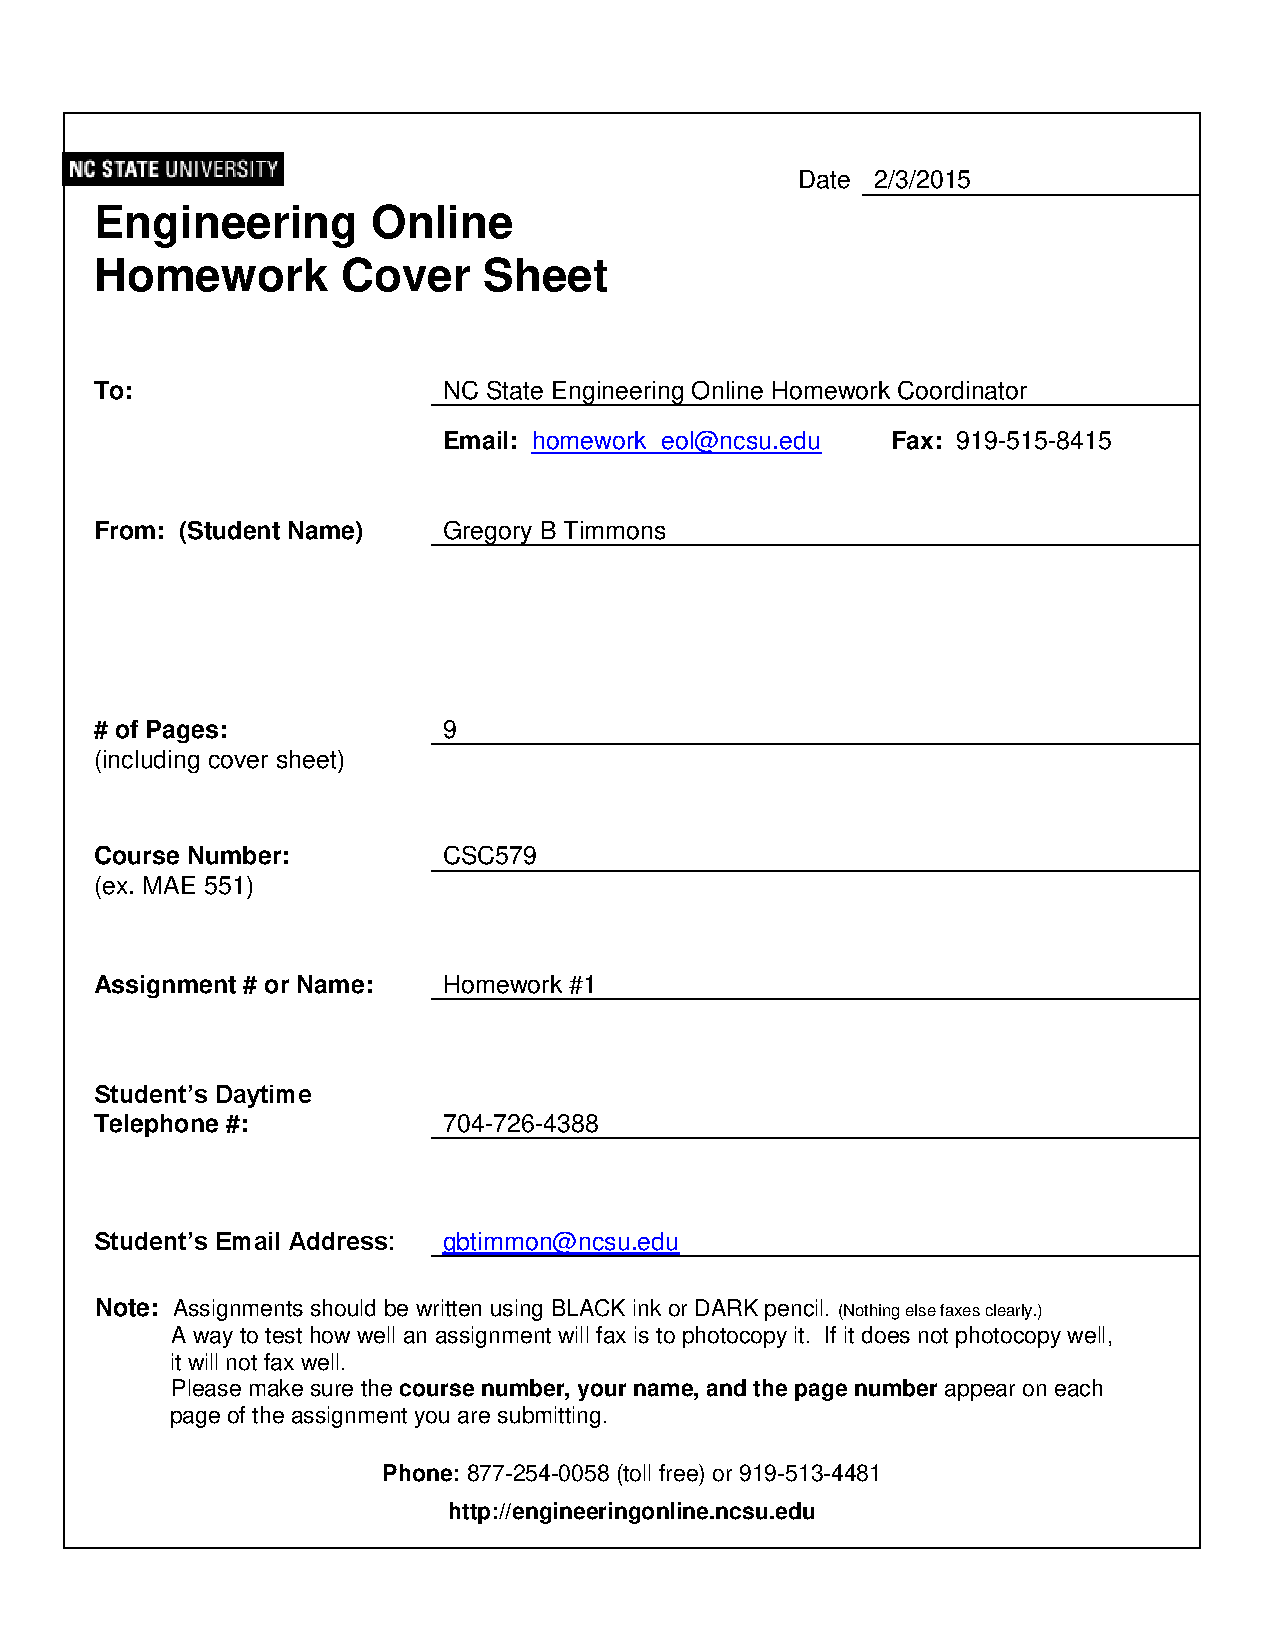
\includepdf[pages={1}]{cover.pdf}
\title{Homework 1}
\date{Febuary 2, 2015}
\author{Gregory B Timmons, gbtimmon}
\maketitle
\begin{document}


\section{Title}

\subsection{Subtitle}

Plain text.

\subsection{Another subtitle}

More plain text.


\end{document}
